Número de ciclos completos que la onda realiza en un segundo. Se representa con la letra $f$ minúscula. Se mide en Hertz $Hz$.

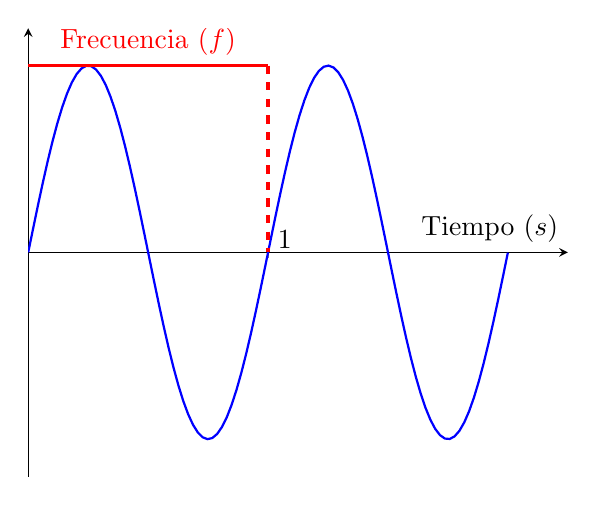
\begin{tikzpicture}
  \begin{axis}[
    xmin=0,xmax=4.5*pi,
    ymin=-1.2,ymax=1.2,
    axis lines=middle,
    xtick={0},
    xtick={2*pi},xticklabels={1},
    xticklabel style={anchor=south west},
    ytick={0},
    xlabel=Tiempo ($s$)
    ]

    % Funcion senoidal
    \addplot[color=blue,samples=100,domain=0:4*pi,thick]{sin(deg(x))};

    % Frecuencia
    \draw[red,thick] (axis cs:0,1) -- (axis cs:2*pi,1) node[pos=0.5,above] {Frecuencia ($f$)};

    % Linea vertical
    \draw[red,dashed,very thick] (axis cs:2*pi,1) -- (axis cs:2*pi,0);
  \end{axis}
\end{tikzpicture}

La frecuencia es el inverso del periodo.

\begin{listequbox}
  {f = \dfrac{1}{T}}{equfrecuencia}{Relación entre frecuencia y periodo}
\end{listequbox}

Interpretando la ecuación \ref{equfrecuencia} en sentido contrario, el periodo es el inverso de la frecuencia.

\[\boxed{
  T = \dfrac{1}{f}
}\]

Teniendo en cuenta el número de ciclos y el periodo en segundos, se puede definir la frecuencia como la cantidad de ciclos por segundo

Considerando esta relación, la unidad de medida de la frecuencia es $\dfrac{1}{s}$ o $s^{-1}$. Esto equivale a un Hertz $Hz$.

\[\boxed{
  \dfrac{1}{s}=s^{-1}=Hz
}\]
